\documentclass[twoside]{book}

% Packages required by doxygen
\usepackage{calc}
\usepackage{doxygen}
\usepackage{graphicx}
\usepackage[utf8]{inputenc}
\usepackage{makeidx}
\usepackage{multicol}
\usepackage{multirow}
\usepackage{textcomp}
\usepackage[table]{xcolor}

% Font selection
\usepackage[T1]{fontenc}
\usepackage{mathptmx}
\usepackage[scaled=.90]{helvet}
\usepackage{courier}
\usepackage{amssymb}
\usepackage{sectsty}
\renewcommand{\familydefault}{\sfdefault}
\allsectionsfont{%
  \fontseries{bc}\selectfont%
  \color{darkgray}%
}
\renewcommand{\DoxyLabelFont}{%
  \fontseries{bc}\selectfont%
  \color{darkgray}%
}

% Page & text layout
\usepackage{geometry}
\geometry{%
  a4paper,%
  top=2.5cm,%
  bottom=2.5cm,%
  left=2.5cm,%
  right=2.5cm%
}
\tolerance=750
\hfuzz=15pt
\hbadness=750
\setlength{\emergencystretch}{15pt}
\setlength{\parindent}{0cm}
\setlength{\parskip}{0.2cm}
\makeatletter
\renewcommand{\paragraph}{%
  \@startsection{paragraph}{4}{0ex}{-1.0ex}{1.0ex}{%
    \normalfont\normalsize\bfseries\SS@parafont%
  }%
}
\renewcommand{\subparagraph}{%
  \@startsection{subparagraph}{5}{0ex}{-1.0ex}{1.0ex}{%
    \normalfont\normalsize\bfseries\SS@subparafont%
  }%
}
\makeatother

% Headers & footers
\usepackage{fancyhdr}
\pagestyle{fancyplain}
\fancyhead[LE]{\fancyplain{}{\bfseries\thepage}}
\fancyhead[CE]{\fancyplain{}{}}
\fancyhead[RE]{\fancyplain{}{\bfseries\leftmark}}
\fancyhead[LO]{\fancyplain{}{\bfseries\rightmark}}
\fancyhead[CO]{\fancyplain{}{}}
\fancyhead[RO]{\fancyplain{}{\bfseries\thepage}}
\fancyfoot[LE]{\fancyplain{}{}}
\fancyfoot[CE]{\fancyplain{}{}}
\fancyfoot[RE]{\fancyplain{}{\bfseries\scriptsize Generated on Mon Feb 10 2014 18\-:25\-:08 for cocos2dx-\/cpp-\/\-I\-F by Doxygen }}
\fancyfoot[LO]{\fancyplain{}{\bfseries\scriptsize Generated on Mon Feb 10 2014 18\-:25\-:08 for cocos2dx-\/cpp-\/\-I\-F by Doxygen }}
\fancyfoot[CO]{\fancyplain{}{}}
\fancyfoot[RO]{\fancyplain{}{}}
\renewcommand{\footrulewidth}{0.4pt}
\renewcommand{\chaptermark}[1]{%
  \markboth{#1}{}%
}
\renewcommand{\sectionmark}[1]{%
  \markright{\thesection\ #1}%
}

% Indices & bibliography
\usepackage{natbib}
\usepackage[titles]{tocloft}
\setcounter{tocdepth}{3}
\setcounter{secnumdepth}{5}
\makeindex

% Hyperlinks (required, but should be loaded last)
\usepackage{ifpdf}
\ifpdf
  \usepackage[pdftex,pagebackref=true]{hyperref}
\else
  \usepackage[ps2pdf,pagebackref=true]{hyperref}
\fi
\hypersetup{%
  colorlinks=true,%
  linkcolor=blue,%
  citecolor=blue,%
  unicode%
}

% Custom commands
\newcommand{\clearemptydoublepage}{%
  \newpage{\pagestyle{empty}\cleardoublepage}%
}


%===== C O N T E N T S =====

\begin{document}

% Titlepage & ToC
\hypersetup{pageanchor=false}
\pagenumbering{roman}
\begin{titlepage}
\vspace*{7cm}
\begin{center}%
{\Large cocos2dx-\/cpp-\/\-I\-F }\\
\vspace*{1cm}
{\large Generated by Doxygen 1.8.6}\\
\vspace*{0.5cm}
{\small Mon Feb 10 2014 18:25:08}\\
\end{center}
\end{titlepage}
\clearemptydoublepage
\tableofcontents
\clearemptydoublepage
\pagenumbering{arabic}
\hypersetup{pageanchor=true}

%--- Begin generated contents ---
\chapter{Hierarchical Index}
\section{Class Hierarchy}
This inheritance list is sorted roughly, but not completely, alphabetically\-:\begin{DoxyCompactList}
\item \contentsline{section}{C\-Kii\-Clause}{\pageref{class_c_kii_clause}}{}
\item \contentsline{section}{C\-Kii\-Query}{\pageref{class_c_kii_query}}{}
\item \contentsline{section}{K\-Base}{\pageref{class_k_base}}{}
\begin{DoxyCompactList}
\item \contentsline{section}{C\-Kii\-Bucket}{\pageref{class_c_kii_bucket}}{}
\end{DoxyCompactList}
\end{DoxyCompactList}

\chapter{Class Index}
\section{Class List}
Here are the classes, structs, unions and interfaces with brief descriptions\-:\begin{DoxyCompactList}
\item\contentsline{section}{\hyperlink{class_c_kii_api_test}{C\-Kii\-Api\-Test} }{\pageref{class_c_kii_api_test}}{}
\item\contentsline{section}{\hyperlink{class_c_kii_bucket}{C\-Kii\-Bucket} }{\pageref{class_c_kii_bucket}}{}
\item\contentsline{section}{\hyperlink{class_c_kii_clause}{C\-Kii\-Clause} }{\pageref{class_c_kii_clause}}{}
\end{DoxyCompactList}

\chapter{Class Documentation}
\hypertarget{class_c_kii_api_test}{\section{C\-Kii\-Api\-Test Class Reference}
\label{class_c_kii_api_test}\index{C\-Kii\-Api\-Test@{C\-Kii\-Api\-Test}}
}
Inheritance diagram for C\-Kii\-Api\-Test\-:\begin{figure}[H]
\begin{center}
\leavevmode
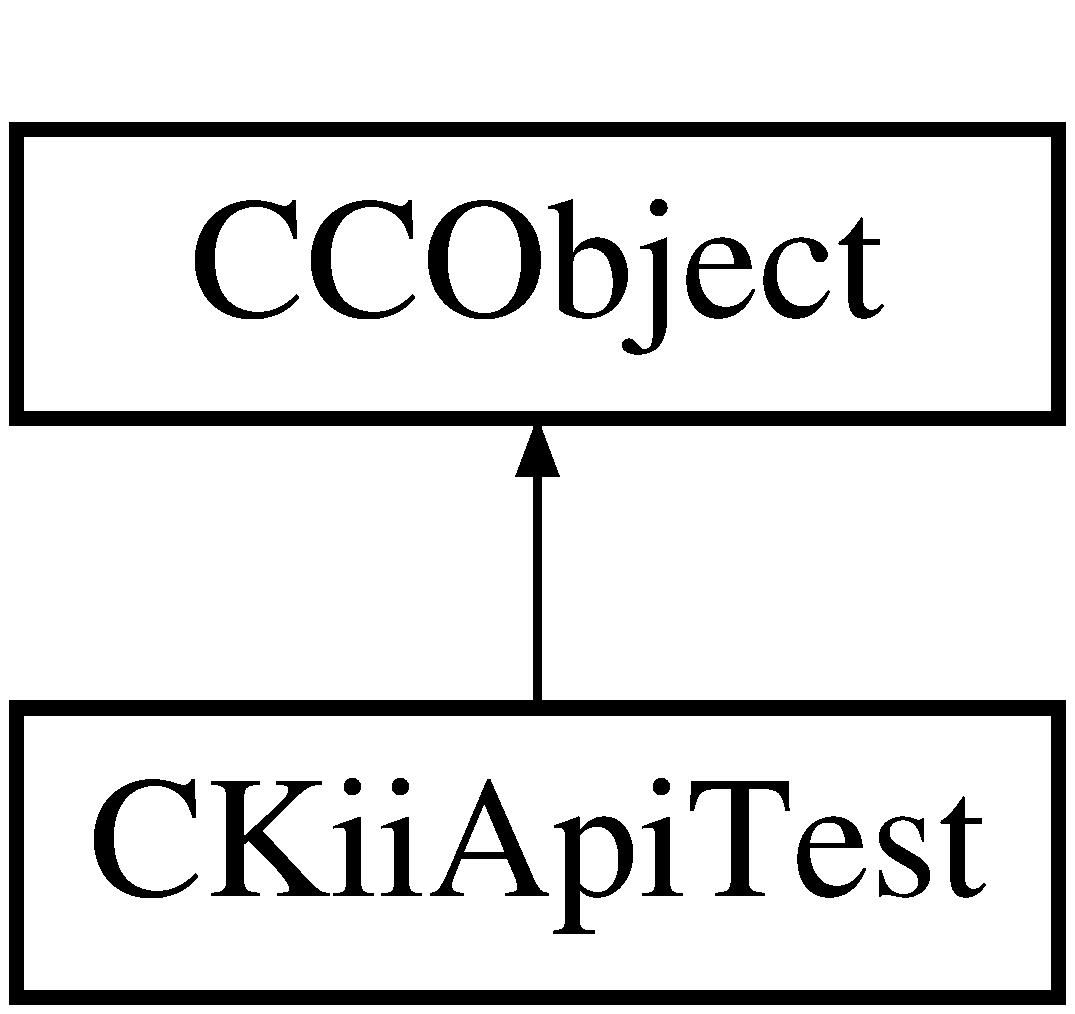
\includegraphics[height=2.000000cm]{class_c_kii_api_test}
\end{center}
\end{figure}
\subsection*{Public Member Functions}
\begin{DoxyCompactItemize}
\item 
\hypertarget{class_c_kii_api_test_ac9326184d44029a868e18ce77ad75890}{bool {\bfseries init} ()}\label{class_c_kii_api_test_ac9326184d44029a868e18ce77ad75890}

\item 
\hypertarget{class_c_kii_api_test_adb2b39d80766474f3259987cdaad2891}{void {\bfseries create\-Application\-Scope\-Bucket\-Test} ()}\label{class_c_kii_api_test_adb2b39d80766474f3259987cdaad2891}

\item 
\hypertarget{class_c_kii_api_test_afc4622e3fe7f3054cc6e4d0cda05a35d}{void {\bfseries call\-Back\-\_\-create\-Application\-Scope\-Bucket\-Test} (const char $\ast$json)}\label{class_c_kii_api_test_afc4622e3fe7f3054cc6e4d0cda05a35d}

\item 
\hypertarget{class_c_kii_api_test_a65020b963779cefb226f66524fd6481f}{void {\bfseries object\-\_\-save\-Test} ()}\label{class_c_kii_api_test_a65020b963779cefb226f66524fd6481f}

\item 
\hypertarget{class_c_kii_api_test_aef8e5dc6b2c1ebc5523601a2bf672cfb}{void {\bfseries call\-Back\-\_\-object\-\_\-save\-Test} (const char $\ast$json)}\label{class_c_kii_api_test_aef8e5dc6b2c1ebc5523601a2bf672cfb}

\item 
\hypertarget{class_c_kii_api_test_a4ac2523bca52b9fe513e7aa27db844e0}{void {\bfseries object\-\_\-refresh\-Test} ()}\label{class_c_kii_api_test_a4ac2523bca52b9fe513e7aa27db844e0}

\item 
\hypertarget{class_c_kii_api_test_aa1b1c7d7687412af8d9167d26ed52459}{void {\bfseries call\-Back\-\_\-object\-\_\-refresh\-Test} (const char $\ast$json)}\label{class_c_kii_api_test_aa1b1c7d7687412af8d9167d26ed52459}

\item 
\hypertarget{class_c_kii_api_test_afa974f9e71dfcb5096b9ac7ac58d3576}{void {\bfseries object\-\_\-update\-Test} ()}\label{class_c_kii_api_test_afa974f9e71dfcb5096b9ac7ac58d3576}

\item 
\hypertarget{class_c_kii_api_test_a1bff468f0ca034e75ccb4d6247baed20}{void {\bfseries call\-Back\-\_\-object\-\_\-update\-Test} (const char $\ast$json)}\label{class_c_kii_api_test_a1bff468f0ca034e75ccb4d6247baed20}

\end{DoxyCompactItemize}
\subsection*{Static Public Member Functions}
\begin{DoxyCompactItemize}
\item 
\hypertarget{class_c_kii_api_test_aa4017a64bbd9c903c257c638d8291ee6}{static \hyperlink{class_c_kii_api_test}{C\-Kii\-Api\-Test} $\ast$ {\bfseries create} ()}\label{class_c_kii_api_test_aa4017a64bbd9c903c257c638d8291ee6}

\end{DoxyCompactItemize}
\subsection*{Public Attributes}
\begin{DoxyCompactItemize}
\item 
\hypertarget{class_c_kii_api_test_a0efcca05f0b3d0f1528a4762257162a6}{\hyperlink{class_c_kii_bucket}{C\-Kii\-Bucket} $\ast$ {\bfseries \-\_\-p\-C\-Kii\-Bucket}}\label{class_c_kii_api_test_a0efcca05f0b3d0f1528a4762257162a6}

\item 
\hypertarget{class_c_kii_api_test_a89ebde6fedb62ffe5ed9f98e52cf6945}{string {\bfseries \-\_\-backet\-\_\-key}}\label{class_c_kii_api_test_a89ebde6fedb62ffe5ed9f98e52cf6945}

\item 
\hypertarget{class_c_kii_api_test_ad39e9b070aca7754a6c754ff5f769594}{string {\bfseries \-\_\-user\-Display\-Name}}\label{class_c_kii_api_test_ad39e9b070aca7754a6c754ff5f769594}

\item 
\hypertarget{class_c_kii_api_test_a2e9cdd55bde457920b81a0a0305e5da3}{string {\bfseries \-\_\-uri}}\label{class_c_kii_api_test_a2e9cdd55bde457920b81a0a0305e5da3}

\item 
\hypertarget{class_c_kii_api_test_a3d774834785707b2870f338cd5a1f60c}{string {\bfseries \-\_\-score}}\label{class_c_kii_api_test_a3d774834785707b2870f338cd5a1f60c}

\item 
\hypertarget{class_c_kii_api_test_aba900d1c916318386b8d6364ac9abf76}{string {\bfseries \-\_\-mode}}\label{class_c_kii_api_test_aba900d1c916318386b8d6364ac9abf76}

\item 
\hypertarget{class_c_kii_api_test_a819ad2cb6fa1387ce02f8c33aee4b8f6}{string {\bfseries \-\_\-premium\-User}}\label{class_c_kii_api_test_a819ad2cb6fa1387ce02f8c33aee4b8f6}

\end{DoxyCompactItemize}


The documentation for this class was generated from the following files\-:\begin{DoxyCompactItemize}
\item 
/\-Users/guest/\-Documents/cocos2d-\/x/cocos2d-\/x-\/2.\-2.\-2/projects/\-My\-App/cocos2dx-\/cpp-\/\-I\-F/\-Classes/kii/C\-Kii\-Api\-Test.\-h\item 
/\-Users/guest/\-Documents/cocos2d-\/x/cocos2d-\/x-\/2.\-2.\-2/projects/\-My\-App/cocos2dx-\/cpp-\/\-I\-F/\-Classes/kii/C\-Kii\-Api\-Test.\-cpp\end{DoxyCompactItemize}

\hypertarget{class_c_kii_bucket}{\section{C\-Kii\-Bucket Class Reference}
\label{class_c_kii_bucket}\index{C\-Kii\-Bucket@{C\-Kii\-Bucket}}
}
Inheritance diagram for C\-Kii\-Bucket\-:\begin{figure}[H]
\begin{center}
\leavevmode
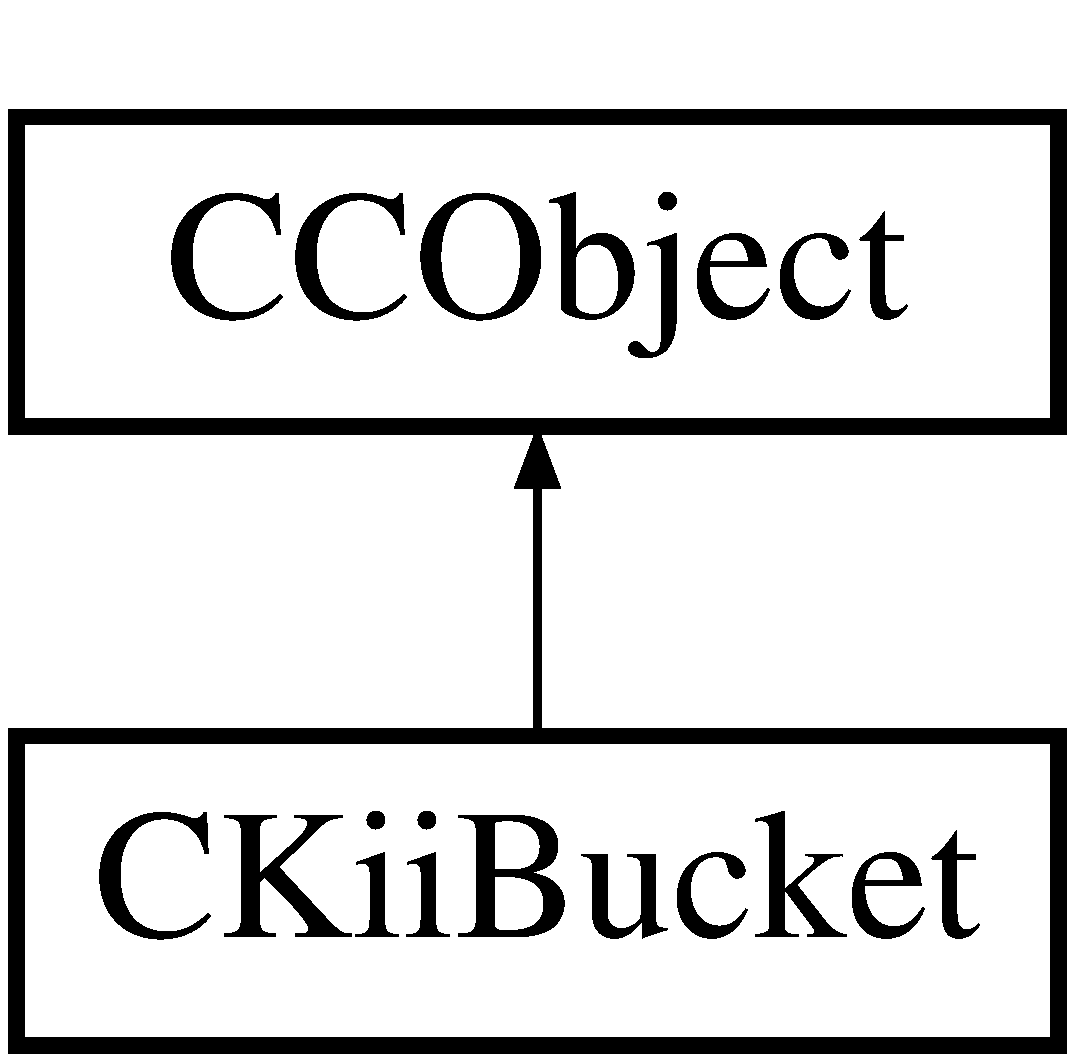
\includegraphics[height=2.000000cm]{class_c_kii_bucket}
\end{center}
\end{figure}
\subsection*{Public Member Functions}
\begin{DoxyCompactItemize}
\item 
bool \hyperlink{class_c_kii_bucket_ae687c3b2a7e95b6e425303c9d944d35b}{init} ()
\begin{DoxyCompactList}\small\item\em 初期化処理 \end{DoxyCompactList}\item 
\hypertarget{class_c_kii_bucket_a63a646fde8ce92f4ba9bc0f1d4b1579c}{void {\bfseries callback} (const char $\ast$json, \hyperlink{class_k_object}{K\-Object} $\ast$target, S\-E\-L\-\_\-callback\-Handler selector)}\label{class_c_kii_bucket_a63a646fde8ce92f4ba9bc0f1d4b1579c}

\item 
void \hyperlink{class_c_kii_bucket_ab469cdd29a09d88b656e04f558a6f5ad}{create\-Application\-Scope\-Bucket} (string backet\-\_\-key, \hyperlink{class_k_object}{K\-Object} $\ast$target, S\-E\-L\-\_\-callback\-Handler selector)
\begin{DoxyCompactList}\small\item\em バケットを作成する(\-Application Scope) \end{DoxyCompactList}\item 
\hypertarget{class_c_kii_bucket_a260a88c89b192ba5cf2c64b5a99d7dac}{void {\bfseries call\-Back\-\_\-create\-Application\-Scope\-Bucket} (const char $\ast$json)}\label{class_c_kii_bucket_a260a88c89b192ba5cf2c64b5a99d7dac}

\item 
void \hyperlink{class_c_kii_bucket_a6a4b9cbfff06eea73a11735c171398b1}{create\-Group\-Scope\-Bucket} (string backet\-\_\-key, \hyperlink{class_k_object}{K\-Object} $\ast$target, S\-E\-L\-\_\-callback\-Handler selector)
\begin{DoxyCompactList}\small\item\em バケットを作成する(\-Group Scope) \end{DoxyCompactList}\item 
\hypertarget{class_c_kii_bucket_a7838074f46d59130d0950df5a3ff4753}{void {\bfseries call\-Back\-\_\-create\-Group\-Scope\-Bucket} (const char $\ast$json)}\label{class_c_kii_bucket_a7838074f46d59130d0950df5a3ff4753}

\item 
void \hyperlink{class_c_kii_bucket_aacf69c6348937433c8582710c5d25931}{create\-User\-Scope\-Bucket} (string backet\-\_\-key, \hyperlink{class_k_object}{K\-Object} $\ast$target, S\-E\-L\-\_\-callback\-Handler selector)
\begin{DoxyCompactList}\small\item\em バケットを作成する(\-User Scope) \end{DoxyCompactList}\item 
\hypertarget{class_c_kii_bucket_a7b2b01aac65959c483b6eefd628b9ae8}{void {\bfseries call\-Back\-\_\-create\-User\-Scope\-Bucket} (const char $\ast$json)}\label{class_c_kii_bucket_a7b2b01aac65959c483b6eefd628b9ae8}

\item 
void \hyperlink{class_c_kii_bucket_af968ac6a7a4d75a7c0ce413a142388cc}{object\-\_\-save} (picojson\-::object key\-\_\-value\-\_\-pairs, \hyperlink{class_k_object}{K\-Object} $\ast$target, S\-E\-L\-\_\-callback\-Handler selector)
\begin{DoxyCompactList}\small\item\em objectを作成する \end{DoxyCompactList}\item 
\hypertarget{class_c_kii_bucket_a57b3dfbce914b0d8ef38145be32f79b3}{void {\bfseries call\-Back\-\_\-object\-\_\-save} (const char $\ast$json)}\label{class_c_kii_bucket_a57b3dfbce914b0d8ef38145be32f79b3}

\item 
void \hyperlink{class_c_kii_bucket_ab5af39edbe6a0e1a136fb620617b63c0}{object\-\_\-refresh} (string uri, \hyperlink{class_k_object}{K\-Object} $\ast$target, S\-E\-L\-\_\-callback\-Handler selector)
\begin{DoxyCompactList}\small\item\em Objectを取得する \end{DoxyCompactList}\item 
\hypertarget{class_c_kii_bucket_ae5fd5045697030cdce7d004fb7e26bc4}{void {\bfseries call\-Back\-\_\-object\-\_\-refresh} (const char $\ast$json)}\label{class_c_kii_bucket_ae5fd5045697030cdce7d004fb7e26bc4}

\item 
void \hyperlink{class_c_kii_bucket_ae9e9ec58df6859c91c4eab89140867b0}{object\-\_\-update} (string uri, picojson\-::object key\-\_\-value\-\_\-pairs, \hyperlink{class_k_object}{K\-Object} $\ast$target, S\-E\-L\-\_\-callback\-Handler selector)
\begin{DoxyCompactList}\small\item\em Objectの更新 \end{DoxyCompactList}\item 
\hypertarget{class_c_kii_bucket_aca9a0b2e3caf7495711312828632bd8e}{void {\bfseries call\-Back\-\_\-object\-\_\-update} (const char $\ast$json)}\label{class_c_kii_bucket_aca9a0b2e3caf7495711312828632bd8e}

\item 
void \hyperlink{class_c_kii_bucket_a0c67e3094a34addff7f0763e86f72abe}{query} (picojson\-::object key\-\_\-value\-\_\-pairs, \hyperlink{class_k_object}{K\-Object} $\ast$target, S\-E\-L\-\_\-callback\-Handler selector)
\begin{DoxyCompactList}\small\item\em Object の検索 \end{DoxyCompactList}\item 
\hypertarget{class_c_kii_bucket_aa36a27887af9177dc7809da7b723bb47}{void {\bfseries call\-Back\-\_\-query} (const char $\ast$json)}\label{class_c_kii_bucket_aa36a27887af9177dc7809da7b723bb47}

\end{DoxyCompactItemize}
\subsection*{Static Public Member Functions}
\begin{DoxyCompactItemize}
\item 
static \hyperlink{class_c_kii_bucket}{C\-Kii\-Bucket} $\ast$ \hyperlink{class_c_kii_bucket_a282979b68d7540433bfb24a4624702de}{create} ()
\begin{DoxyCompactList}\small\item\em メモリー確保する \end{DoxyCompactList}\end{DoxyCompactItemize}
\subsection*{Public Attributes}
\begin{DoxyCompactItemize}
\item 
\hypertarget{class_c_kii_bucket_ae62e874439f55143f8009f88da23bc99}{string {\bfseries \-\_\-backet\-\_\-key}}\label{class_c_kii_bucket_ae62e874439f55143f8009f88da23bc99}

\item 
\hypertarget{class_c_kii_bucket_aa18c6b0053f2e0a2a07c33e5dc490802}{string {\bfseries \-\_\-uri}}\label{class_c_kii_bucket_aa18c6b0053f2e0a2a07c33e5dc490802}

\item 
\hypertarget{class_c_kii_bucket_abb9c612afef7908a3e03f302aba20480}{\hyperlink{class_k_object}{K\-Object} $\ast$ {\bfseries target\-\_\-create\-Application\-Scope\-Bucket}}\label{class_c_kii_bucket_abb9c612afef7908a3e03f302aba20480}

\item 
\hypertarget{class_c_kii_bucket_a4a5b74eb7eea8c621668c2cd8a5f7cb4}{S\-E\-L\-\_\-callback\-Handler {\bfseries selector\-\_\-create\-Application\-Scope\-Bucket}}\label{class_c_kii_bucket_a4a5b74eb7eea8c621668c2cd8a5f7cb4}

\item 
\hypertarget{class_c_kii_bucket_a262c5942c6c5cc86abb3c4e62d0ea98c}{\hyperlink{class_k_object}{K\-Object} $\ast$ {\bfseries target\-\_\-create\-Group\-Scope\-Bucket}}\label{class_c_kii_bucket_a262c5942c6c5cc86abb3c4e62d0ea98c}

\item 
\hypertarget{class_c_kii_bucket_a0070b496c90629e11bd409d7fe28cbda}{S\-E\-L\-\_\-callback\-Handler {\bfseries selector\-\_\-create\-Group\-Scope\-Bucket}}\label{class_c_kii_bucket_a0070b496c90629e11bd409d7fe28cbda}

\item 
\hypertarget{class_c_kii_bucket_ac35f08bfe1508ca0095b5e3ee6bbb6fb}{\hyperlink{class_k_object}{K\-Object} $\ast$ {\bfseries target\-\_\-create\-User\-Scope\-Bucket}}\label{class_c_kii_bucket_ac35f08bfe1508ca0095b5e3ee6bbb6fb}

\item 
\hypertarget{class_c_kii_bucket_ab596059653bc65a47a98f7dfbbd3f55c}{S\-E\-L\-\_\-callback\-Handler {\bfseries selector\-\_\-create\-User\-Scope\-Bucket}}\label{class_c_kii_bucket_ab596059653bc65a47a98f7dfbbd3f55c}

\item 
\hypertarget{class_c_kii_bucket_a2dc55c811e95dc321e1cb95f1dae0adf}{\hyperlink{class_k_object}{K\-Object} $\ast$ {\bfseries target\-\_\-object\-\_\-save}}\label{class_c_kii_bucket_a2dc55c811e95dc321e1cb95f1dae0adf}

\item 
\hypertarget{class_c_kii_bucket_a90b8bf7cb1cc5ed6c299a574833f3fd2}{S\-E\-L\-\_\-callback\-Handler {\bfseries selector\-\_\-object\-\_\-save}}\label{class_c_kii_bucket_a90b8bf7cb1cc5ed6c299a574833f3fd2}

\item 
\hypertarget{class_c_kii_bucket_ac495e6539bff57eae86f3203ebe06687}{\hyperlink{class_k_object}{K\-Object} $\ast$ {\bfseries target\-\_\-object\-\_\-refresh}}\label{class_c_kii_bucket_ac495e6539bff57eae86f3203ebe06687}

\item 
\hypertarget{class_c_kii_bucket_ac9e641126b3d8315b2b41c55f829190b}{S\-E\-L\-\_\-callback\-Handler {\bfseries selector\-\_\-object\-\_\-refresh}}\label{class_c_kii_bucket_ac9e641126b3d8315b2b41c55f829190b}

\item 
\hypertarget{class_c_kii_bucket_a8e912e1c7d17b102337d61cc87e8a9c0}{\hyperlink{class_k_object}{K\-Object} $\ast$ {\bfseries target\-\_\-object\-\_\-update}}\label{class_c_kii_bucket_a8e912e1c7d17b102337d61cc87e8a9c0}

\item 
\hypertarget{class_c_kii_bucket_ad840394a0cc208a1fd19ba0a0b147f5e}{S\-E\-L\-\_\-callback\-Handler {\bfseries selector\-\_\-object\-\_\-update}}\label{class_c_kii_bucket_ad840394a0cc208a1fd19ba0a0b147f5e}

\item 
\hypertarget{class_c_kii_bucket_aa8045e51b4b1a8923e1d3e5646c856e6}{\hyperlink{class_k_object}{K\-Object} $\ast$ {\bfseries target\-\_\-object\-\_\-query}}\label{class_c_kii_bucket_aa8045e51b4b1a8923e1d3e5646c856e6}

\item 
\hypertarget{class_c_kii_bucket_a32e7019eff0bd1fd6ec1dfce8d03bc5d}{S\-E\-L\-\_\-callback\-Handler {\bfseries selector\-\_\-object\-\_\-query}}\label{class_c_kii_bucket_a32e7019eff0bd1fd6ec1dfce8d03bc5d}

\end{DoxyCompactItemize}


\subsection{Member Function Documentation}
\hypertarget{class_c_kii_bucket_a282979b68d7540433bfb24a4624702de}{\index{C\-Kii\-Bucket@{C\-Kii\-Bucket}!create@{create}}
\index{create@{create}!CKiiBucket@{C\-Kii\-Bucket}}
\subsubsection[{create}]{\setlength{\rightskip}{0pt plus 5cm}{\bf C\-Kii\-Bucket} $\ast$ C\-Kii\-Bucket\-::create (
\begin{DoxyParamCaption}
{}
\end{DoxyParamCaption}
)\hspace{0.3cm}{\ttfamily [static]}}}\label{class_c_kii_bucket_a282979b68d7540433bfb24a4624702de}


メモリー確保する 


\begin{DoxyParams}{Parameters}
{\em @return} & \\
\hline
{\em なし} & \\
\hline
\end{DoxyParams}
\begin{DoxyReturn}{Returns}
オブジェクトのポインター 
\end{DoxyReturn}
\hypertarget{class_c_kii_bucket_ab469cdd29a09d88b656e04f558a6f5ad}{\index{C\-Kii\-Bucket@{C\-Kii\-Bucket}!create\-Application\-Scope\-Bucket@{create\-Application\-Scope\-Bucket}}
\index{create\-Application\-Scope\-Bucket@{create\-Application\-Scope\-Bucket}!CKiiBucket@{C\-Kii\-Bucket}}
\subsubsection[{create\-Application\-Scope\-Bucket}]{\setlength{\rightskip}{0pt plus 5cm}void C\-Kii\-Bucket\-::create\-Application\-Scope\-Bucket (
\begin{DoxyParamCaption}
\item[{string}]{backet\-\_\-key, }
\item[{{\bf K\-Object} $\ast$}]{target, }
\item[{S\-E\-L\-\_\-callback\-Handler}]{selector}
\end{DoxyParamCaption}
)}}\label{class_c_kii_bucket_ab469cdd29a09d88b656e04f558a6f5ad}


バケットを作成する(\-Application Scope) 


\begin{DoxyParams}{Parameters}
{\em backet\-\_\-key} & バケットを識別する文字列 \\
\hline
{\em target} & 呼び出し元のクラスのポインタ \\
\hline
{\em selector} & コールバックメソッドのポインタ \\
\hline
\end{DoxyParams}
\begin{DoxyReturn}{Returns}
backet\-\_\-key バケットを識別する文字列 
\end{DoxyReturn}
\hypertarget{class_c_kii_bucket_a6a4b9cbfff06eea73a11735c171398b1}{\index{C\-Kii\-Bucket@{C\-Kii\-Bucket}!create\-Group\-Scope\-Bucket@{create\-Group\-Scope\-Bucket}}
\index{create\-Group\-Scope\-Bucket@{create\-Group\-Scope\-Bucket}!CKiiBucket@{C\-Kii\-Bucket}}
\subsubsection[{create\-Group\-Scope\-Bucket}]{\setlength{\rightskip}{0pt plus 5cm}void C\-Kii\-Bucket\-::create\-Group\-Scope\-Bucket (
\begin{DoxyParamCaption}
\item[{string}]{backet\-\_\-key, }
\item[{{\bf K\-Object} $\ast$}]{target, }
\item[{S\-E\-L\-\_\-callback\-Handler}]{selector}
\end{DoxyParamCaption}
)}}\label{class_c_kii_bucket_a6a4b9cbfff06eea73a11735c171398b1}


バケットを作成する(\-Group Scope) 


\begin{DoxyParams}{Parameters}
{\em backet\-\_\-key} & バケットを識別する文字列 \\
\hline
{\em target} & 呼び出し元のクラスのポインタ \\
\hline
{\em selector} & コールバックメソッドのポインタ \\
\hline
\end{DoxyParams}
\begin{DoxyReturn}{Returns}
backet\-\_\-key バケットを識別する文字列 
\end{DoxyReturn}
\hypertarget{class_c_kii_bucket_aacf69c6348937433c8582710c5d25931}{\index{C\-Kii\-Bucket@{C\-Kii\-Bucket}!create\-User\-Scope\-Bucket@{create\-User\-Scope\-Bucket}}
\index{create\-User\-Scope\-Bucket@{create\-User\-Scope\-Bucket}!CKiiBucket@{C\-Kii\-Bucket}}
\subsubsection[{create\-User\-Scope\-Bucket}]{\setlength{\rightskip}{0pt plus 5cm}void C\-Kii\-Bucket\-::create\-User\-Scope\-Bucket (
\begin{DoxyParamCaption}
\item[{string}]{backet\-\_\-key, }
\item[{{\bf K\-Object} $\ast$}]{target, }
\item[{S\-E\-L\-\_\-callback\-Handler}]{selector}
\end{DoxyParamCaption}
)}}\label{class_c_kii_bucket_aacf69c6348937433c8582710c5d25931}


バケットを作成する(\-User Scope) 


\begin{DoxyParams}{Parameters}
{\em backet\-\_\-key} & バケットを識別する文字列 \\
\hline
{\em target} & 呼び出し元のクラスのポインタ \\
\hline
{\em selector} & コールバックメソッドのポインタ \\
\hline
\end{DoxyParams}
\begin{DoxyReturn}{Returns}
backet\-\_\-key バケットを識別する文字列 
\end{DoxyReturn}
\hypertarget{class_c_kii_bucket_ae687c3b2a7e95b6e425303c9d944d35b}{\index{C\-Kii\-Bucket@{C\-Kii\-Bucket}!init@{init}}
\index{init@{init}!CKiiBucket@{C\-Kii\-Bucket}}
\subsubsection[{init}]{\setlength{\rightskip}{0pt plus 5cm}bool C\-Kii\-Bucket\-::init (
\begin{DoxyParamCaption}
{}
\end{DoxyParamCaption}
)}}\label{class_c_kii_bucket_ae687c3b2a7e95b6e425303c9d944d35b}


初期化処理 


\begin{DoxyParams}{Parameters}
{\em なし} & \\
\hline
\end{DoxyParams}
\begin{DoxyReturn}{Returns}
成功or失敗 
\end{DoxyReturn}
\hypertarget{class_c_kii_bucket_ab5af39edbe6a0e1a136fb620617b63c0}{\index{C\-Kii\-Bucket@{C\-Kii\-Bucket}!object\-\_\-refresh@{object\-\_\-refresh}}
\index{object\-\_\-refresh@{object\-\_\-refresh}!CKiiBucket@{C\-Kii\-Bucket}}
\subsubsection[{object\-\_\-refresh}]{\setlength{\rightskip}{0pt plus 5cm}void C\-Kii\-Bucket\-::object\-\_\-refresh (
\begin{DoxyParamCaption}
\item[{string}]{uri, }
\item[{{\bf K\-Object} $\ast$}]{target, }
\item[{S\-E\-L\-\_\-callback\-Handler}]{selector}
\end{DoxyParamCaption}
)}}\label{class_c_kii_bucket_ab5af39edbe6a0e1a136fb620617b63c0}


Objectを取得する 


\begin{DoxyParams}{Parameters}
{\em uri} & オブジェクトを特定するuri文字列 \\
\hline
{\em target} & 呼び出し元のクラスのポインタ \\
\hline
{\em selector} & コールバックメソッドのポインタ \\
\hline
\end{DoxyParams}
\begin{DoxyReturn}{Returns}
なし、別途コールバックより返る 
\end{DoxyReturn}
\hypertarget{class_c_kii_bucket_af968ac6a7a4d75a7c0ce413a142388cc}{\index{C\-Kii\-Bucket@{C\-Kii\-Bucket}!object\-\_\-save@{object\-\_\-save}}
\index{object\-\_\-save@{object\-\_\-save}!CKiiBucket@{C\-Kii\-Bucket}}
\subsubsection[{object\-\_\-save}]{\setlength{\rightskip}{0pt plus 5cm}void C\-Kii\-Bucket\-::object\-\_\-save (
\begin{DoxyParamCaption}
\item[{picojson\-::object}]{key\-\_\-value\-\_\-pairs, }
\item[{{\bf K\-Object} $\ast$}]{target, }
\item[{S\-E\-L\-\_\-callback\-Handler}]{selector}
\end{DoxyParamCaption}
)}}\label{class_c_kii_bucket_af968ac6a7a4d75a7c0ce413a142388cc}


objectを作成する 


\begin{DoxyParams}{Parameters}
{\em key\-\_\-value\-\_\-pairs} & 保存する key-\/valueのpair \\
\hline
{\em target} & 呼び出し元のクラスのポインタ \\
\hline
{\em selector} & コールバックメソッドのポインタ \\
\hline
\end{DoxyParams}
\begin{DoxyReturn}{Returns}
なし、別途コールバックより返る 
\end{DoxyReturn}
\hypertarget{class_c_kii_bucket_ae9e9ec58df6859c91c4eab89140867b0}{\index{C\-Kii\-Bucket@{C\-Kii\-Bucket}!object\-\_\-update@{object\-\_\-update}}
\index{object\-\_\-update@{object\-\_\-update}!CKiiBucket@{C\-Kii\-Bucket}}
\subsubsection[{object\-\_\-update}]{\setlength{\rightskip}{0pt plus 5cm}void C\-Kii\-Bucket\-::object\-\_\-update (
\begin{DoxyParamCaption}
\item[{string}]{uri, }
\item[{picojson\-::object}]{key\-\_\-value\-\_\-pairs, }
\item[{{\bf K\-Object} $\ast$}]{target, }
\item[{S\-E\-L\-\_\-callback\-Handler}]{selector}
\end{DoxyParamCaption}
)}}\label{class_c_kii_bucket_ae9e9ec58df6859c91c4eab89140867b0}


Objectの更新 


\begin{DoxyParams}{Parameters}
{\em } & オブジェクトを特定するuri文字列 \\
\hline
{\em key\-\_\-value\-\_\-pairs} & 更新するkey-\/valueのpair \\
\hline
{\em target} & 呼び出し元のクラスのポインタ \\
\hline
{\em selector} & コールバックメソッドのポインタ \\
\hline
\end{DoxyParams}
\begin{DoxyReturn}{Returns}
なし、別途コールバックより返る 
\end{DoxyReturn}
\hypertarget{class_c_kii_bucket_a0c67e3094a34addff7f0763e86f72abe}{\index{C\-Kii\-Bucket@{C\-Kii\-Bucket}!query@{query}}
\index{query@{query}!CKiiBucket@{C\-Kii\-Bucket}}
\subsubsection[{query}]{\setlength{\rightskip}{0pt plus 5cm}void C\-Kii\-Bucket\-::query (
\begin{DoxyParamCaption}
\item[{picojson\-::object}]{key\-\_\-value\-\_\-pairs, }
\item[{{\bf K\-Object} $\ast$}]{target, }
\item[{S\-E\-L\-\_\-callback\-Handler}]{selector}
\end{DoxyParamCaption}
)}}\label{class_c_kii_bucket_a0c67e3094a34addff7f0763e86f72abe}


Object の検索 


\begin{DoxyParams}{Parameters}
{\em query} & ソート条件等 \\
\hline
{\em clause} & 検索条件 \\
\hline
\end{DoxyParams}
\begin{DoxyReturn}{Returns}
なし、別途コールバックより返る 
\end{DoxyReturn}


The documentation for this class was generated from the following files\-:\begin{DoxyCompactItemize}
\item 
/\-Users/guest/\-Documents/cocos2d-\/x/cocos2d-\/x-\/2.\-2.\-2/projects/\-My\-App/cocos2dx-\/cpp-\/\-I\-F/\-Classes/kii/C\-Kii\-Bucket.\-h\item 
/\-Users/guest/\-Documents/cocos2d-\/x/cocos2d-\/x-\/2.\-2.\-2/projects/\-My\-App/cocos2dx-\/cpp-\/\-I\-F/\-Classes/kii/C\-Kii\-Bucket.\-cpp\end{DoxyCompactItemize}

\hypertarget{class_c_kii_clause}{\section{C\-Kii\-Clause Class Reference}
\label{class_c_kii_clause}\index{C\-Kii\-Clause@{C\-Kii\-Clause}}
}
\subsection*{Static Public Member Functions}
\begin{DoxyCompactItemize}
\item 
static std\-::shared\-\_\-ptr\\*
$<$ \hyperlink{class_c_kii_clause}{C\-Kii\-Clause} $>$ \hyperlink{class_c_kii_clause_a31aa4b7f40cde23d8da1eefc69089a10}{equals} (const string \&key, int value)
\begin{DoxyCompactList}\small\item\em equals フィールド値が、指定の値に等しい場合にマッチ。 \end{DoxyCompactList}\item 
static std\-::shared\-\_\-ptr\\*
$<$ \hyperlink{class_c_kii_clause}{C\-Kii\-Clause} $>$ \hyperlink{class_c_kii_clause_a7b1e1efd3ebf56c6ca619ee66b9ee2ab}{equals} (const string \&key, double value)
\begin{DoxyCompactList}\small\item\em equals フィールド値が、指定の値に等しい場合にマッチ。 \end{DoxyCompactList}\item 
static std\-::shared\-\_\-ptr\\*
$<$ \hyperlink{class_c_kii_clause}{C\-Kii\-Clause} $>$ \hyperlink{class_c_kii_clause_a514ad24cf5ace4f80e4d4eac4dd7166a}{equals} (const string \&key, const string \&value)
\begin{DoxyCompactList}\small\item\em equals フィールド値が、指定の値に等しい場合にマッチ。 \end{DoxyCompactList}\item 
static std\-::shared\-\_\-ptr\\*
$<$ \hyperlink{class_c_kii_clause}{C\-Kii\-Clause} $>$ \hyperlink{class_c_kii_clause_a14e15cd786186cdd0de6a988b1271c7d}{not\-Equals} (const string \&key, int value)
\begin{DoxyCompactList}\small\item\em not\-Equals フィールド値が、指定の値に等しくない場合にマッチ。 \end{DoxyCompactList}\item 
static std\-::shared\-\_\-ptr\\*
$<$ \hyperlink{class_c_kii_clause}{C\-Kii\-Clause} $>$ \hyperlink{class_c_kii_clause_a852def0f04ce641ecb34691c30763803}{not\-Equals} (const string \&key, double value)
\begin{DoxyCompactList}\small\item\em not\-Equals フィールド値が、指定の値に等しくない場合にマッチ。 \end{DoxyCompactList}\item 
static std\-::shared\-\_\-ptr\\*
$<$ \hyperlink{class_c_kii_clause}{C\-Kii\-Clause} $>$ \hyperlink{class_c_kii_clause_af581fa5e81a7003eacf27cda974ec119}{not\-Equals} (const string \&key, const string \&value)
\begin{DoxyCompactList}\small\item\em not\-Equals フィールド値が、指定の値に等しくない場合にマッチ。 \end{DoxyCompactList}\item 
static std\-::shared\-\_\-ptr\\*
$<$ \hyperlink{class_c_kii_clause}{C\-Kii\-Clause} $>$ \hyperlink{class_c_kii_clause_ab3e8e71ab31fa53efa7c828516325cc0}{greater\-Than} (const string \&key, int value)
\begin{DoxyCompactList}\small\item\em not\-Equals フィールド値が、指定の値より大きい場合にマッチ。 \end{DoxyCompactList}\item 
static std\-::shared\-\_\-ptr\\*
$<$ \hyperlink{class_c_kii_clause}{C\-Kii\-Clause} $>$ \hyperlink{class_c_kii_clause_a782d42431601d16608f99070ef347c6b}{greater\-Than} (const string \&key, double value)
\begin{DoxyCompactList}\small\item\em greater\-Than フィールド値が、指定の値より大きい場合にマッチ。 \end{DoxyCompactList}\item 
static std\-::shared\-\_\-ptr\\*
$<$ \hyperlink{class_c_kii_clause}{C\-Kii\-Clause} $>$ \hyperlink{class_c_kii_clause_a7f36064e49d85516c86b915ff20402b9}{greater\-Than} (const string \&key, const string \&value)
\begin{DoxyCompactList}\small\item\em フィールド値が、指定の値より大きい場合にマッチ。 \end{DoxyCompactList}\item 
static std\-::shared\-\_\-ptr\\*
$<$ \hyperlink{class_c_kii_clause}{C\-Kii\-Clause} $>$ \hyperlink{class_c_kii_clause_af2e77eb171a8abef023211d92a418f2c}{greater\-Than\-Or\-Equal} (const string \&key, int value)
\begin{DoxyCompactList}\small\item\em フィールド値が、指定の値以上の場合にマッチ。 \end{DoxyCompactList}\item 
static std\-::shared\-\_\-ptr\\*
$<$ \hyperlink{class_c_kii_clause}{C\-Kii\-Clause} $>$ \hyperlink{class_c_kii_clause_ab051c9136381a6b42b411101aee2069e}{greater\-Than\-Or\-Equal} (const string \&key, double value)
\begin{DoxyCompactList}\small\item\em フィールド値が、指定の値以上の場合にマッチ。 \end{DoxyCompactList}\item 
static std\-::shared\-\_\-ptr\\*
$<$ \hyperlink{class_c_kii_clause}{C\-Kii\-Clause} $>$ \hyperlink{class_c_kii_clause_a349c83b0e32f0133103c731667db5518}{greater\-Than\-Or\-Equal} (const string \&key, const string \&value)
\begin{DoxyCompactList}\small\item\em フィールド値が、指定の値以上の場合にマッチ。 \end{DoxyCompactList}\item 
static std\-::shared\-\_\-ptr\\*
$<$ \hyperlink{class_c_kii_clause}{C\-Kii\-Clause} $>$ \hyperlink{class_c_kii_clause_a8d485b3e6c354985dfdb9925387da4d9}{less\-Than} (const string \&key, int value)
\begin{DoxyCompactList}\small\item\em フィールド値が、指定の値より小さい場合にマッチ。 \end{DoxyCompactList}\item 
static std\-::shared\-\_\-ptr\\*
$<$ \hyperlink{class_c_kii_clause}{C\-Kii\-Clause} $>$ \hyperlink{class_c_kii_clause_af61bde1e5bf272d9bb97d53d47b04c7f}{less\-Than} (const string \&key, double value)
\begin{DoxyCompactList}\small\item\em フィールド値が、指定の値より小さい場合にマッチ。 \end{DoxyCompactList}\item 
static std\-::shared\-\_\-ptr\\*
$<$ \hyperlink{class_c_kii_clause}{C\-Kii\-Clause} $>$ \hyperlink{class_c_kii_clause_a80f180f1d69c2e99a59060ad5baaa4fa}{less\-Than} (const string \&key, const string \&value)
\begin{DoxyCompactList}\small\item\em フィールド値が、指定の値より小さい場合にマッチ。 \end{DoxyCompactList}\item 
static std\-::shared\-\_\-ptr\\*
$<$ \hyperlink{class_c_kii_clause}{C\-Kii\-Clause} $>$ \hyperlink{class_c_kii_clause_aac4fe1a687424ffd518d8ac4938b07e9}{less\-Than\-Or\-Equal} (const string \&key, int value)
\begin{DoxyCompactList}\small\item\em フィールド値が、指定の値以下の場合にマッチ。 \end{DoxyCompactList}\item 
static std\-::shared\-\_\-ptr\\*
$<$ \hyperlink{class_c_kii_clause}{C\-Kii\-Clause} $>$ \hyperlink{class_c_kii_clause_aa1112eff242879f56e8ff01a2d2a0158}{less\-Than\-Or\-Equal} (const string \&key, double value)
\begin{DoxyCompactList}\small\item\em フィールド値が、指定の値以下の場合にマッチ。 \end{DoxyCompactList}\item 
static std\-::shared\-\_\-ptr\\*
$<$ \hyperlink{class_c_kii_clause}{C\-Kii\-Clause} $>$ \hyperlink{class_c_kii_clause_ac261d6021b7c3bc7e3b872cbd15f7e87}{less\-Than\-Or\-Equal} (const string \&key, const string \&value)
\begin{DoxyCompactList}\small\item\em フィールド値が、指定の値以下の場合にマッチ。 \end{DoxyCompactList}\item 
static std\-::shared\-\_\-ptr\\*
$<$ \hyperlink{class_c_kii_clause}{C\-Kii\-Clause} $>$ \hyperlink{class_c_kii_clause_aa8ffe90a53af7db170cc0861847e681f}{starts\-With} (const string \&key, const string \&value)
\begin{DoxyCompactList}\small\item\em フィールド値 (String 型) が、指定の文字列により始まっている場合にマッチ。 \end{DoxyCompactList}\item 
static std\-::shared\-\_\-ptr\\*
$<$ \hyperlink{class_c_kii_clause}{C\-Kii\-Clause} $>$ \hyperlink{class_c_kii_clause_a1838a01e387edbaefc828be5904cd603}{\-\_\-or} (int num,...)
\begin{DoxyCompactList}\small\item\em 複数の検索条件を O\-R で結合。 \end{DoxyCompactList}\item 
static std\-::shared\-\_\-ptr\\*
$<$ \hyperlink{class_c_kii_clause}{C\-Kii\-Clause} $>$ \hyperlink{class_c_kii_clause_a5a41ba6dc119a7eb023052842d1ab27c}{\-\_\-and} (int num,...)
\begin{DoxyCompactList}\small\item\em 複数の検索条件を A\-N\-D で結合。 \end{DoxyCompactList}\end{DoxyCompactItemize}
\subsection*{Public Attributes}
\begin{DoxyCompactItemize}
\item 
\hypertarget{class_c_kii_clause_acfc92615decf8779aedf763ea81eefd6}{picojson\-::object {\bfseries \-\_\-json}}\label{class_c_kii_clause_acfc92615decf8779aedf763ea81eefd6}

\end{DoxyCompactItemize}


\subsection{Member Function Documentation}
\hypertarget{class_c_kii_clause_a5a41ba6dc119a7eb023052842d1ab27c}{\index{C\-Kii\-Clause@{C\-Kii\-Clause}!\-\_\-and@{\-\_\-and}}
\index{\-\_\-and@{\-\_\-and}!CKiiClause@{C\-Kii\-Clause}}
\subsubsection[{\-\_\-and}]{\setlength{\rightskip}{0pt plus 5cm}std\-::shared\-\_\-ptr$<$ {\bf C\-Kii\-Clause} $>$ C\-Kii\-Clause\-::\-\_\-and (
\begin{DoxyParamCaption}
\item[{int}]{num, }
\item[{}]{...}
\end{DoxyParamCaption}
)\hspace{0.3cm}{\ttfamily [static]}}}\label{class_c_kii_clause_a5a41ba6dc119a7eb023052842d1ab27c}


複数の検索条件を A\-N\-D で結合。 


\begin{DoxyParams}{Parameters}
{\em int} & andで渡す引数の数 \\
\hline
{\em andの条件} & \\
\hline
\end{DoxyParams}
\begin{DoxyReturn}{Returns}
given clause. 
\end{DoxyReturn}
\hypertarget{class_c_kii_clause_a1838a01e387edbaefc828be5904cd603}{\index{C\-Kii\-Clause@{C\-Kii\-Clause}!\-\_\-or@{\-\_\-or}}
\index{\-\_\-or@{\-\_\-or}!CKiiClause@{C\-Kii\-Clause}}
\subsubsection[{\-\_\-or}]{\setlength{\rightskip}{0pt plus 5cm}std\-::shared\-\_\-ptr$<$ {\bf C\-Kii\-Clause} $>$ C\-Kii\-Clause\-::\-\_\-or (
\begin{DoxyParamCaption}
\item[{int}]{num, }
\item[{}]{...}
\end{DoxyParamCaption}
)\hspace{0.3cm}{\ttfamily [static]}}}\label{class_c_kii_clause_a1838a01e387edbaefc828be5904cd603}


複数の検索条件を O\-R で結合。 


\begin{DoxyParams}{Parameters}
{\em int} & orで渡す引数の数 \\
\hline
{\em orの条件} & \\
\hline
\end{DoxyParams}
\begin{DoxyReturn}{Returns}
given clause. 
\end{DoxyReturn}
\hypertarget{class_c_kii_clause_a31aa4b7f40cde23d8da1eefc69089a10}{\index{C\-Kii\-Clause@{C\-Kii\-Clause}!equals@{equals}}
\index{equals@{equals}!CKiiClause@{C\-Kii\-Clause}}
\subsubsection[{equals}]{\setlength{\rightskip}{0pt plus 5cm}std\-::shared\-\_\-ptr$<$ {\bf C\-Kii\-Clause} $>$ C\-Kii\-Clause\-::equals (
\begin{DoxyParamCaption}
\item[{const string \&}]{key, }
\item[{int}]{value}
\end{DoxyParamCaption}
)\hspace{0.3cm}{\ttfamily [static]}}}\label{class_c_kii_clause_a31aa4b7f40cde23d8da1eefc69089a10}


equals フィールド値が、指定の値に等しい場合にマッチ。 


\begin{DoxyParams}{Parameters}
{\em key} & target of comparison. \\
\hline
{\em value} & to be compared. \\
\hline
\end{DoxyParams}
\begin{DoxyReturn}{Returns}
std\-::shared\-\_\-ptr$<$\-C\-Kii\-Clause$>$ instance. 
\end{DoxyReturn}
\hypertarget{class_c_kii_clause_a7b1e1efd3ebf56c6ca619ee66b9ee2ab}{\index{C\-Kii\-Clause@{C\-Kii\-Clause}!equals@{equals}}
\index{equals@{equals}!CKiiClause@{C\-Kii\-Clause}}
\subsubsection[{equals}]{\setlength{\rightskip}{0pt plus 5cm}std\-::shared\-\_\-ptr$<$ {\bf C\-Kii\-Clause} $>$ C\-Kii\-Clause\-::equals (
\begin{DoxyParamCaption}
\item[{const string \&}]{key, }
\item[{double}]{value}
\end{DoxyParamCaption}
)\hspace{0.3cm}{\ttfamily [static]}}}\label{class_c_kii_clause_a7b1e1efd3ebf56c6ca619ee66b9ee2ab}


equals フィールド値が、指定の値に等しい場合にマッチ。 


\begin{DoxyParams}{Parameters}
{\em key} & target of comparison. \\
\hline
{\em value} & to be compared. \\
\hline
\end{DoxyParams}
\begin{DoxyReturn}{Returns}
std\-::shared\-\_\-ptr$<$\-C\-Kii\-Clause$>$ instance. 
\end{DoxyReturn}
\hypertarget{class_c_kii_clause_a514ad24cf5ace4f80e4d4eac4dd7166a}{\index{C\-Kii\-Clause@{C\-Kii\-Clause}!equals@{equals}}
\index{equals@{equals}!CKiiClause@{C\-Kii\-Clause}}
\subsubsection[{equals}]{\setlength{\rightskip}{0pt plus 5cm}std\-::shared\-\_\-ptr$<$ {\bf C\-Kii\-Clause} $>$ C\-Kii\-Clause\-::equals (
\begin{DoxyParamCaption}
\item[{const string \&}]{key, }
\item[{const string \&}]{value}
\end{DoxyParamCaption}
)\hspace{0.3cm}{\ttfamily [static]}}}\label{class_c_kii_clause_a514ad24cf5ace4f80e4d4eac4dd7166a}


equals フィールド値が、指定の値に等しい場合にマッチ。 


\begin{DoxyParams}{Parameters}
{\em key} & target of comparison. \\
\hline
{\em value} & to be compared. \\
\hline
\end{DoxyParams}
\begin{DoxyReturn}{Returns}
std\-::shared\-\_\-ptr$<$\-C\-Kii\-Clause$>$ instance. 
\end{DoxyReturn}
\hypertarget{class_c_kii_clause_ab3e8e71ab31fa53efa7c828516325cc0}{\index{C\-Kii\-Clause@{C\-Kii\-Clause}!greater\-Than@{greater\-Than}}
\index{greater\-Than@{greater\-Than}!CKiiClause@{C\-Kii\-Clause}}
\subsubsection[{greater\-Than}]{\setlength{\rightskip}{0pt plus 5cm}std\-::shared\-\_\-ptr$<$ {\bf C\-Kii\-Clause} $>$ C\-Kii\-Clause\-::greater\-Than (
\begin{DoxyParamCaption}
\item[{const string \&}]{key, }
\item[{int}]{value}
\end{DoxyParamCaption}
)\hspace{0.3cm}{\ttfamily [static]}}}\label{class_c_kii_clause_ab3e8e71ab31fa53efa7c828516325cc0}


not\-Equals フィールド値が、指定の値より大きい場合にマッチ。 


\begin{DoxyParams}{Parameters}
{\em key} & target of comparison. \\
\hline
{\em value} & to be compared. \\
\hline
\end{DoxyParams}
\begin{DoxyReturn}{Returns}
std\-::shared\-\_\-ptr$<$\-C\-Kii\-Clause$>$ instance. 
\end{DoxyReturn}
\hypertarget{class_c_kii_clause_a782d42431601d16608f99070ef347c6b}{\index{C\-Kii\-Clause@{C\-Kii\-Clause}!greater\-Than@{greater\-Than}}
\index{greater\-Than@{greater\-Than}!CKiiClause@{C\-Kii\-Clause}}
\subsubsection[{greater\-Than}]{\setlength{\rightskip}{0pt plus 5cm}std\-::shared\-\_\-ptr$<$ {\bf C\-Kii\-Clause} $>$ C\-Kii\-Clause\-::greater\-Than (
\begin{DoxyParamCaption}
\item[{const string \&}]{key, }
\item[{double}]{value}
\end{DoxyParamCaption}
)\hspace{0.3cm}{\ttfamily [static]}}}\label{class_c_kii_clause_a782d42431601d16608f99070ef347c6b}


greater\-Than フィールド値が、指定の値より大きい場合にマッチ。 


\begin{DoxyParams}{Parameters}
{\em key} & target of comparison. \\
\hline
{\em value} & to be compared. \\
\hline
\end{DoxyParams}
\begin{DoxyReturn}{Returns}
std\-::shared\-\_\-ptr$<$\-C\-Kii\-Clause$>$ instance. 
\end{DoxyReturn}
\hypertarget{class_c_kii_clause_a7f36064e49d85516c86b915ff20402b9}{\index{C\-Kii\-Clause@{C\-Kii\-Clause}!greater\-Than@{greater\-Than}}
\index{greater\-Than@{greater\-Than}!CKiiClause@{C\-Kii\-Clause}}
\subsubsection[{greater\-Than}]{\setlength{\rightskip}{0pt plus 5cm}std\-::shared\-\_\-ptr$<$ {\bf C\-Kii\-Clause} $>$ C\-Kii\-Clause\-::greater\-Than (
\begin{DoxyParamCaption}
\item[{const string \&}]{key, }
\item[{const string \&}]{value}
\end{DoxyParamCaption}
)\hspace{0.3cm}{\ttfamily [static]}}}\label{class_c_kii_clause_a7f36064e49d85516c86b915ff20402b9}


フィールド値が、指定の値より大きい場合にマッチ。 


\begin{DoxyParams}{Parameters}
{\em key} & target of comparison. \\
\hline
{\em value} & to be compared. \\
\hline
\end{DoxyParams}
\begin{DoxyReturn}{Returns}
std\-::shared\-\_\-ptr$<$\-C\-Kii\-Clause$>$ instance. 
\end{DoxyReturn}
\hypertarget{class_c_kii_clause_af2e77eb171a8abef023211d92a418f2c}{\index{C\-Kii\-Clause@{C\-Kii\-Clause}!greater\-Than\-Or\-Equal@{greater\-Than\-Or\-Equal}}
\index{greater\-Than\-Or\-Equal@{greater\-Than\-Or\-Equal}!CKiiClause@{C\-Kii\-Clause}}
\subsubsection[{greater\-Than\-Or\-Equal}]{\setlength{\rightskip}{0pt plus 5cm}std\-::shared\-\_\-ptr$<$ {\bf C\-Kii\-Clause} $>$ C\-Kii\-Clause\-::greater\-Than\-Or\-Equal (
\begin{DoxyParamCaption}
\item[{const string \&}]{key, }
\item[{int}]{value}
\end{DoxyParamCaption}
)\hspace{0.3cm}{\ttfamily [static]}}}\label{class_c_kii_clause_af2e77eb171a8abef023211d92a418f2c}


フィールド値が、指定の値以上の場合にマッチ。 


\begin{DoxyParams}{Parameters}
{\em key} & target of comparison. \\
\hline
{\em value} & to be compared. \\
\hline
\end{DoxyParams}
\begin{DoxyReturn}{Returns}
std\-::shared\-\_\-ptr$<$\-C\-Kii\-Clause$>$ instance. 
\end{DoxyReturn}
\hypertarget{class_c_kii_clause_ab051c9136381a6b42b411101aee2069e}{\index{C\-Kii\-Clause@{C\-Kii\-Clause}!greater\-Than\-Or\-Equal@{greater\-Than\-Or\-Equal}}
\index{greater\-Than\-Or\-Equal@{greater\-Than\-Or\-Equal}!CKiiClause@{C\-Kii\-Clause}}
\subsubsection[{greater\-Than\-Or\-Equal}]{\setlength{\rightskip}{0pt plus 5cm}std\-::shared\-\_\-ptr$<$ {\bf C\-Kii\-Clause} $>$ C\-Kii\-Clause\-::greater\-Than\-Or\-Equal (
\begin{DoxyParamCaption}
\item[{const string \&}]{key, }
\item[{double}]{value}
\end{DoxyParamCaption}
)\hspace{0.3cm}{\ttfamily [static]}}}\label{class_c_kii_clause_ab051c9136381a6b42b411101aee2069e}


フィールド値が、指定の値以上の場合にマッチ。 


\begin{DoxyParams}{Parameters}
{\em key} & target of comparison. \\
\hline
{\em value} & to be compared. \\
\hline
\end{DoxyParams}
\begin{DoxyReturn}{Returns}
std\-::shared\-\_\-ptr$<$\-C\-Kii\-Clause$>$ instance. 
\end{DoxyReturn}
\hypertarget{class_c_kii_clause_a349c83b0e32f0133103c731667db5518}{\index{C\-Kii\-Clause@{C\-Kii\-Clause}!greater\-Than\-Or\-Equal@{greater\-Than\-Or\-Equal}}
\index{greater\-Than\-Or\-Equal@{greater\-Than\-Or\-Equal}!CKiiClause@{C\-Kii\-Clause}}
\subsubsection[{greater\-Than\-Or\-Equal}]{\setlength{\rightskip}{0pt plus 5cm}std\-::shared\-\_\-ptr$<$ {\bf C\-Kii\-Clause} $>$ C\-Kii\-Clause\-::greater\-Than\-Or\-Equal (
\begin{DoxyParamCaption}
\item[{const string \&}]{key, }
\item[{const string \&}]{value}
\end{DoxyParamCaption}
)\hspace{0.3cm}{\ttfamily [static]}}}\label{class_c_kii_clause_a349c83b0e32f0133103c731667db5518}


フィールド値が、指定の値以上の場合にマッチ。 


\begin{DoxyParams}{Parameters}
{\em key} & target of comparison. \\
\hline
{\em value} & to be compared. \\
\hline
\end{DoxyParams}
\begin{DoxyReturn}{Returns}
std\-::shared\-\_\-ptr$<$\-C\-Kii\-Clause$>$ instance. 
\end{DoxyReturn}
\hypertarget{class_c_kii_clause_a8d485b3e6c354985dfdb9925387da4d9}{\index{C\-Kii\-Clause@{C\-Kii\-Clause}!less\-Than@{less\-Than}}
\index{less\-Than@{less\-Than}!CKiiClause@{C\-Kii\-Clause}}
\subsubsection[{less\-Than}]{\setlength{\rightskip}{0pt plus 5cm}std\-::shared\-\_\-ptr$<$ {\bf C\-Kii\-Clause} $>$ C\-Kii\-Clause\-::less\-Than (
\begin{DoxyParamCaption}
\item[{const string \&}]{key, }
\item[{int}]{value}
\end{DoxyParamCaption}
)\hspace{0.3cm}{\ttfamily [static]}}}\label{class_c_kii_clause_a8d485b3e6c354985dfdb9925387da4d9}


フィールド値が、指定の値より小さい場合にマッチ。 


\begin{DoxyParams}{Parameters}
{\em key} & target of comparison. \\
\hline
{\em value} & to be compared. \\
\hline
\end{DoxyParams}
\begin{DoxyReturn}{Returns}
std\-::shared\-\_\-ptr$<$\-C\-Kii\-Clause$>$ instance. 
\end{DoxyReturn}
\hypertarget{class_c_kii_clause_af61bde1e5bf272d9bb97d53d47b04c7f}{\index{C\-Kii\-Clause@{C\-Kii\-Clause}!less\-Than@{less\-Than}}
\index{less\-Than@{less\-Than}!CKiiClause@{C\-Kii\-Clause}}
\subsubsection[{less\-Than}]{\setlength{\rightskip}{0pt plus 5cm}std\-::shared\-\_\-ptr$<$ {\bf C\-Kii\-Clause} $>$ C\-Kii\-Clause\-::less\-Than (
\begin{DoxyParamCaption}
\item[{const string \&}]{key, }
\item[{double}]{value}
\end{DoxyParamCaption}
)\hspace{0.3cm}{\ttfamily [static]}}}\label{class_c_kii_clause_af61bde1e5bf272d9bb97d53d47b04c7f}


フィールド値が、指定の値より小さい場合にマッチ。 


\begin{DoxyParams}{Parameters}
{\em key} & target of comparison. \\
\hline
{\em value} & to be compared. \\
\hline
\end{DoxyParams}
\begin{DoxyReturn}{Returns}
std\-::shared\-\_\-ptr$<$\-C\-Kii\-Clause$>$ instance. 
\end{DoxyReturn}
\hypertarget{class_c_kii_clause_a80f180f1d69c2e99a59060ad5baaa4fa}{\index{C\-Kii\-Clause@{C\-Kii\-Clause}!less\-Than@{less\-Than}}
\index{less\-Than@{less\-Than}!CKiiClause@{C\-Kii\-Clause}}
\subsubsection[{less\-Than}]{\setlength{\rightskip}{0pt plus 5cm}std\-::shared\-\_\-ptr$<$ {\bf C\-Kii\-Clause} $>$ C\-Kii\-Clause\-::less\-Than (
\begin{DoxyParamCaption}
\item[{const string \&}]{key, }
\item[{const string \&}]{value}
\end{DoxyParamCaption}
)\hspace{0.3cm}{\ttfamily [static]}}}\label{class_c_kii_clause_a80f180f1d69c2e99a59060ad5baaa4fa}


フィールド値が、指定の値より小さい場合にマッチ。 


\begin{DoxyParams}{Parameters}
{\em key} & target of comparison. \\
\hline
{\em value} & to be compared. \\
\hline
\end{DoxyParams}
\begin{DoxyReturn}{Returns}
std\-::shared\-\_\-ptr$<$\-C\-Kii\-Clause$>$ instance. 
\end{DoxyReturn}
\hypertarget{class_c_kii_clause_aac4fe1a687424ffd518d8ac4938b07e9}{\index{C\-Kii\-Clause@{C\-Kii\-Clause}!less\-Than\-Or\-Equal@{less\-Than\-Or\-Equal}}
\index{less\-Than\-Or\-Equal@{less\-Than\-Or\-Equal}!CKiiClause@{C\-Kii\-Clause}}
\subsubsection[{less\-Than\-Or\-Equal}]{\setlength{\rightskip}{0pt plus 5cm}std\-::shared\-\_\-ptr$<$ {\bf C\-Kii\-Clause} $>$ C\-Kii\-Clause\-::less\-Than\-Or\-Equal (
\begin{DoxyParamCaption}
\item[{const string \&}]{key, }
\item[{int}]{value}
\end{DoxyParamCaption}
)\hspace{0.3cm}{\ttfamily [static]}}}\label{class_c_kii_clause_aac4fe1a687424ffd518d8ac4938b07e9}


フィールド値が、指定の値以下の場合にマッチ。 


\begin{DoxyParams}{Parameters}
{\em key} & target of comparison. \\
\hline
{\em value} & to be compared. \\
\hline
\end{DoxyParams}
\begin{DoxyReturn}{Returns}
std\-::shared\-\_\-ptr$<$\-C\-Kii\-Clause$>$ instance. 
\end{DoxyReturn}
\hypertarget{class_c_kii_clause_aa1112eff242879f56e8ff01a2d2a0158}{\index{C\-Kii\-Clause@{C\-Kii\-Clause}!less\-Than\-Or\-Equal@{less\-Than\-Or\-Equal}}
\index{less\-Than\-Or\-Equal@{less\-Than\-Or\-Equal}!CKiiClause@{C\-Kii\-Clause}}
\subsubsection[{less\-Than\-Or\-Equal}]{\setlength{\rightskip}{0pt plus 5cm}std\-::shared\-\_\-ptr$<$ {\bf C\-Kii\-Clause} $>$ C\-Kii\-Clause\-::less\-Than\-Or\-Equal (
\begin{DoxyParamCaption}
\item[{const string \&}]{key, }
\item[{double}]{value}
\end{DoxyParamCaption}
)\hspace{0.3cm}{\ttfamily [static]}}}\label{class_c_kii_clause_aa1112eff242879f56e8ff01a2d2a0158}


フィールド値が、指定の値以下の場合にマッチ。 


\begin{DoxyParams}{Parameters}
{\em key} & target of comparison. \\
\hline
{\em value} & to be compared. \\
\hline
\end{DoxyParams}
\begin{DoxyReturn}{Returns}
std\-::shared\-\_\-ptr$<$\-C\-Kii\-Clause$>$ instance. 
\end{DoxyReturn}
\hypertarget{class_c_kii_clause_ac261d6021b7c3bc7e3b872cbd15f7e87}{\index{C\-Kii\-Clause@{C\-Kii\-Clause}!less\-Than\-Or\-Equal@{less\-Than\-Or\-Equal}}
\index{less\-Than\-Or\-Equal@{less\-Than\-Or\-Equal}!CKiiClause@{C\-Kii\-Clause}}
\subsubsection[{less\-Than\-Or\-Equal}]{\setlength{\rightskip}{0pt plus 5cm}std\-::shared\-\_\-ptr$<$ {\bf C\-Kii\-Clause} $>$ C\-Kii\-Clause\-::less\-Than\-Or\-Equal (
\begin{DoxyParamCaption}
\item[{const string \&}]{key, }
\item[{const string \&}]{value}
\end{DoxyParamCaption}
)\hspace{0.3cm}{\ttfamily [static]}}}\label{class_c_kii_clause_ac261d6021b7c3bc7e3b872cbd15f7e87}


フィールド値が、指定の値以下の場合にマッチ。 


\begin{DoxyParams}{Parameters}
{\em key} & target of comparison. \\
\hline
{\em value} & to be compared. \\
\hline
\end{DoxyParams}
\begin{DoxyReturn}{Returns}
std\-::shared\-\_\-ptr$<$\-C\-Kii\-Clause$>$ instance. 
\end{DoxyReturn}
\hypertarget{class_c_kii_clause_a14e15cd786186cdd0de6a988b1271c7d}{\index{C\-Kii\-Clause@{C\-Kii\-Clause}!not\-Equals@{not\-Equals}}
\index{not\-Equals@{not\-Equals}!CKiiClause@{C\-Kii\-Clause}}
\subsubsection[{not\-Equals}]{\setlength{\rightskip}{0pt plus 5cm}std\-::shared\-\_\-ptr$<$ {\bf C\-Kii\-Clause} $>$ C\-Kii\-Clause\-::not\-Equals (
\begin{DoxyParamCaption}
\item[{const string \&}]{key, }
\item[{int}]{value}
\end{DoxyParamCaption}
)\hspace{0.3cm}{\ttfamily [static]}}}\label{class_c_kii_clause_a14e15cd786186cdd0de6a988b1271c7d}


not\-Equals フィールド値が、指定の値に等しくない場合にマッチ。 


\begin{DoxyParams}{Parameters}
{\em key} & target of comparison. \\
\hline
{\em value} & to be compared. \\
\hline
\end{DoxyParams}
\begin{DoxyReturn}{Returns}
std\-::shared\-\_\-ptr$<$\-C\-Kii\-Clause$>$ instance. 
\end{DoxyReturn}
\hypertarget{class_c_kii_clause_a852def0f04ce641ecb34691c30763803}{\index{C\-Kii\-Clause@{C\-Kii\-Clause}!not\-Equals@{not\-Equals}}
\index{not\-Equals@{not\-Equals}!CKiiClause@{C\-Kii\-Clause}}
\subsubsection[{not\-Equals}]{\setlength{\rightskip}{0pt plus 5cm}std\-::shared\-\_\-ptr$<$ {\bf C\-Kii\-Clause} $>$ C\-Kii\-Clause\-::not\-Equals (
\begin{DoxyParamCaption}
\item[{const string \&}]{key, }
\item[{double}]{value}
\end{DoxyParamCaption}
)\hspace{0.3cm}{\ttfamily [static]}}}\label{class_c_kii_clause_a852def0f04ce641ecb34691c30763803}


not\-Equals フィールド値が、指定の値に等しくない場合にマッチ。 


\begin{DoxyParams}{Parameters}
{\em key} & target of comparison. \\
\hline
{\em value} & to be compared. \\
\hline
\end{DoxyParams}
\begin{DoxyReturn}{Returns}
std\-::shared\-\_\-ptr$<$\-C\-Kii\-Clause$>$ instance. 
\end{DoxyReturn}
\hypertarget{class_c_kii_clause_af581fa5e81a7003eacf27cda974ec119}{\index{C\-Kii\-Clause@{C\-Kii\-Clause}!not\-Equals@{not\-Equals}}
\index{not\-Equals@{not\-Equals}!CKiiClause@{C\-Kii\-Clause}}
\subsubsection[{not\-Equals}]{\setlength{\rightskip}{0pt plus 5cm}std\-::shared\-\_\-ptr$<$ {\bf C\-Kii\-Clause} $>$ C\-Kii\-Clause\-::not\-Equals (
\begin{DoxyParamCaption}
\item[{const string \&}]{key, }
\item[{const string \&}]{value}
\end{DoxyParamCaption}
)\hspace{0.3cm}{\ttfamily [static]}}}\label{class_c_kii_clause_af581fa5e81a7003eacf27cda974ec119}


not\-Equals フィールド値が、指定の値に等しくない場合にマッチ。 


\begin{DoxyParams}{Parameters}
{\em key} & target of comparison. \\
\hline
{\em value} & to be compared. \\
\hline
\end{DoxyParams}
\begin{DoxyReturn}{Returns}
std\-::shared\-\_\-ptr$<$\-C\-Kii\-Clause$>$ instance. 
\end{DoxyReturn}
\hypertarget{class_c_kii_clause_aa8ffe90a53af7db170cc0861847e681f}{\index{C\-Kii\-Clause@{C\-Kii\-Clause}!starts\-With@{starts\-With}}
\index{starts\-With@{starts\-With}!CKiiClause@{C\-Kii\-Clause}}
\subsubsection[{starts\-With}]{\setlength{\rightskip}{0pt plus 5cm}std\-::shared\-\_\-ptr$<$ {\bf C\-Kii\-Clause} $>$ C\-Kii\-Clause\-::starts\-With (
\begin{DoxyParamCaption}
\item[{const string \&}]{key, }
\item[{const string \&}]{value}
\end{DoxyParamCaption}
)\hspace{0.3cm}{\ttfamily [static]}}}\label{class_c_kii_clause_aa8ffe90a53af7db170cc0861847e681f}


フィールド値 (String 型) が、指定の文字列により始まっている場合にマッチ。 


\begin{DoxyParams}{Parameters}
{\em key} & target of comparison. \\
\hline
{\em value} & to be compared. \\
\hline
\end{DoxyParams}
\begin{DoxyReturn}{Returns}
Kistd\-::shared\-\_\-ptr$<$\-C\-Kii\-Clause$>$i\-Clause instance. 
\end{DoxyReturn}


The documentation for this class was generated from the following files\-:\begin{DoxyCompactItemize}
\item 
C\-Kii\-Clause.\-h\item 
C\-Kii\-Clause.\-cpp\end{DoxyCompactItemize}

%--- End generated contents ---

% Index
\newpage
\phantomsection
\addcontentsline{toc}{chapter}{Index}
\printindex

\end{document}
